
\section{Raggiungibilità ed osservabilità}
Queste due proprietà cercano di studiare in modo qualitativo le potenzialità
dell'ingresso di un certo sistema ISU e la possibilità che offre l'uscita
rispetto alla possibilità di capire cosa accade nel sistema osservando l'uscita.
Le potenzialità dell'ingresso possono influenzare l'evoluzione dello stato,
racchiuso in un sottospazio $X^n$ dell'intero sistema, non è infatti detto che
l'ingresso possa modificare senza vincoli tutte le variabili di stato, questo
fenomeno viene studiato attraverso la proprietà di raggiungibilità.

Si vuole inoltre capire se è possibile ricostruire l'evoluzione interna dello
stato attraverso l'osservazione dell'uscita, in generale non è possibile, si può
ricostruire una parte dello stato e non tutto.

\subsection{Raggiungibilità (LTI)}
Uno stato $\hat{x}$ è raggiungibile se e solo se
$$
\hat{x} \text{ raggiungibile} \Leftrightarrow  \exists \hat{t},
\hat{u}_{[t_0,\hat{t}]} : \left.x_f(\hat{t})\right|_{u=\hat{u}} = \hat{x}
$$
esiste un tempo $\hat{t}$ ed un ingresso $\hat{u}$ tali per cui l'evoluzione
forzata $x_f(\hat{t})$ coincida con lo stato $\hat{x}$.
Questa caratteristica equivale a dire che è possibile pilotare il sistema
mediante l'ingresso in un certo intervallo finito e portarlo proprio nello
stato desiderato.
Un sistema in cui tutti gli stati sono raggiungibili si dirà
\textit{completamente raggiungibile}, si definisce il sottospazio di
raggiungibilità $X_R$ sottoinsieme dello spazio dello stato.
$$
X_R = \{ x\in X^n : x \text{ è raggiungibile}\} \subseteq X^n
$$
Se il sottospazio di raggiungibilità coincide con lo spazio dello stato allora
il sistema nella sua forma ISU è completamente raggiungibile.
La raggiungibilità è fondamentale per un progettista, permette di capire se si
hanno a disposizione i giusti ingressi per il sistema in esame e per
modificarne lo stato.

Si consideri la funzione della risposta forzata dalle formule di Lagrange
$$
x_f(t) = \int_{t_0}^t e^{A(t-t_0)}Bu(\tau) d\tau
$$
Nell'espressione compaiono solo le matrici $A$ e $B$, dunque la proprietà di
raggiungibilità dipende solo da queste due matrici. La matrice $A$ contiene i
modi naturali e le caratteristiche interne al sistema, la matrice $B$ invece
modula l'ingresso e lo lega alla variabile di stato.

Un drone ad esempio è un sistema sottoattuato, non si può controllare
istantaneamente la sua posizione e il suo orientamento ma si possono solo
comandare i motori e quindi la spinta risultante, non si può in alcun modo
applicare una spinta (senza aggiungere ulteriori eliche e dunque variabili di
ingresso) che sia ortogonale al piano del drone.

\subsubsection{Matrice di raggiungibilità}
Permette di studiare la raggiungibilità del sistema, è una matrice a blocchi
per colonna, il primo blocco è la matrice $B$, poi il prodotto di $A\times B$
fino ad $A^{n-1}B$ dove $n$ è la dimensione del sistema (o della matrice $A$)
$$
R=\left(\begin{array}{c|c|c|c|c}
   B & AB & A^2B & \dots & A^{n-1}B
  \end{array}\right)\qquad n\times(n\cdot m )
$$
Uno stato $\hat{x}$ è raggiungibile se e solo se
$$
\hat{x} \text{ raggiungibile} \Leftrightarrow \hat{x} \in X_R =
\text{Immagine}\{R\}
$$
Un sistema è completamente raggiungibile se $X_R$ corrisponde a tutto lo spazio
$X^n$ ma ciò è vero se la matrice $R$ è di ragno pieno.
Per i sistemi con un solo ingresso la matrice diventa quadrata, è sufficiente
assicurarsi che il determinante sia diverso da zero affinchè abbia rango
massimo.

Si consideri il seguente esempio
$$
A = \begin{pmatrix}
     1 & 2 \\
     1 & 2
    \end{pmatrix}
\quad B = \begin{pmatrix}
           1 \\ 1
          \end{pmatrix} \longrightarrow
R=
\begin{array}{c}
B \ AB \\
\left(\begin{array}{c:c}
    1 & 3 \\
    1 & 3
   \end{array}\right)
\end{array}\quad
\rho(R) = 1 < 2
$$
Il sottospazio di raggiungibilità $X_R$ non coincide con tutto lo spazio di
stato, si deve ricavare la base associata alla matrice $R$ estraendo le colonne
linearmente indipendenti, in questo caso è sufficiente usare la prima colonna
$$
\text{Immagine}\{R\} = <\begin{bmatrix}
                         1 \\ 1
                        \end{bmatrix}>
$$
Lo spazio ha dimensione 2 $(n=2)$ mentre la base ha dimensione 1, dunque il
sottospazio di raggiungibilità è la retta passante per l'origine degli assi
dello stato con pendenza unitaria.
Ciò significa che si può fornire al sistema un ingresso qualsiasi ma lo stato
sarà vincolato a muoversi solo lungo la retta $X_R$ ossia tale che $x_1=x_2$
qualunque sia l'ingresso.
La proprietà di raggiungibilità è una proprietà differenziale, non dipende
dalla durata dell'ingresso, se pure si fornisse un ingresso per un tempo
inferiore, al limite infinitesimo, aumentando l'ampiezza dell'ingresso, al
limite impulsivo, si otterrebbe comunque uno stato pari al prodotto $Bu(t)$.

Per capire quali parti dello stato sono raggiungibili e quali non lo sono,
è necessario eseguire una trasformazione di similitudine mediante una matrice,
ci si pone nell'ipotesi $\rho(R) = n_r<n$ altrimenti il sistema sarebbe
completamente raggiungibile, esiste un'intera classe di matrici $T_R$
invertibili
$$
\rho(R) = n_r<n \Rightarrow \exists T_R \text{ invertibile} : x=T_rz
$$
dunque le matrici $A$ e $B$ diventano
$$
A_R = T_R^{-1} A T_R = \begin{pmatrix}
                        A_{11} & A_{12} \\
                        0 & A_{22}
                       \end{pmatrix}
\qquad
B_R = \begin{pmatrix}
       B_1 \\ 0
      \end{pmatrix} = T_R^{-1}B
$$
Si otterranno delle matrici a blocchi triangolari superiori, la matrice
$A_{11}$ di dimensioni $n_r \times n_r$ mentre la $B_1$ sarà $n_r \times m$

La matrice C diventa
$$
C_R = CT_r = \begin{pmatrix}
              C_1 & C_2
             \end{pmatrix}
$$
Il nuovo sistema ISU diventa
$$
\left\{\begin{aligned}
\dot{z} &= A_R z + B_R u \\
y &= C_Rz + Du
\end{aligned}\right.
$$
Si partizione il vettore $z$ chiamando i suoi primi $n_R$ elementi $Z_1$ e i
restanti $n-n_R$ si chiameranno $Z_2$.
$$
z = \begin{pmatrix}
Z_1 \\ Z_2
\end{pmatrix}
$$

Il sistema così partizionato assume la seguente struttura
$$
\left\{\begin{aligned}
\dot{Z}_1 &= A_{11}Z_1 + A_{12} Z_2 + B_1 u\\
\dot{Z}_2 &= A_{22}Z_2\\
y &= C_1Z_1 + C_2 Z_2 +Du
\end{aligned}\right.
$$
Si mostra una rappresentazione grafica del sistema, può essere visto suddiviso
in due sottosistemi, il primo associato alla prima equazione differenziale e il
secondo alla seconda.
Per il primo sottosistema la matrice $A_{11}$ coincide alla sua matrice della
dinamica, dipende dallo stato $Z_1$ mentre la matrice $A_{12}$ rappresenta la
mutua relazione tra il sottosistema $Z_1$ e l'ingresso $Z_2$ fornito dal
rispettivo sottosistema, dunque $Z_2$ può essere considerato come un ingresso
per il sottosistema $Z_1$.
Il sottosistema $Z_2$ è autonomo, non ha ingressi, dunque non è raggiungibile.
\begin{figure}[h]
 \centering
 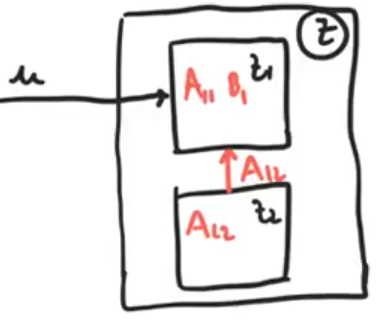
\includegraphics[width=\picwid]{sistema_raggiungibile}
\end{figure}

Si dimostra che la coppia $(A_{11},B_1)$ è completamente raggiungibile
$$
\rho({R}) = \rho\left(B_R,\ A_RB_R\ \dots\ A_R^{n-1}B_R\right) = \rho
\begin{pmatrix}
B_1 & A_{11}B_1 & \ldots & A_{11}^{n-1}B_1\\
 0  &     0     &        &   0
\end{pmatrix}
\stackrel{\text{ipotesi}}{=}n_R
$$

La prima riga della matrice $R$ contiene $n_R$ righe per costruzione, dato che
il rango è massimo allora tutte le colonne saranno linearmente indipendenti tra
loro ma queste colonne formano proprio la matrice di raggiungibilità del
sottosistema 1, dunque esso è completamente raggiungibile.

La matrice della dinamica è triangolare alta, dunque i suoi autovalori sono gli
autovalori dei blocchi sulla diagonale, ossia di $A_{11}$ e $A_{22}$ ma i primi
appartengono alla parte raggiungibile, quelli di $A_{22}$ no.

La matrice $T_R$ deve essere invertibile, si costruisce nel seguente modo: si
inseriscono $n_R$ colonne linearmente indipendenti tali che siano una base di
$X_R$ possono essere prese dalla matrice di raggiungibilità $R$ ed
eventualmente combinarle affinché siano ancora una base, si completa la matrice
$T_R$ con $n-n_R$ colonne arbitrarie, rispettando sempre il vincolo del
determinante di $T_R\neq 0$
57:45
